\documentclass[a4paper,utf8]{article}
\usepackage{graphicx}
\usepackage{graphicx}
\usepackage[heading,fancyhdr]{ctex}
\usepackage{amsmath,amssymb,geometry,ulem}
\usepackage{array,tabularx,tabulary,mhchem,xspace}
\usepackage{floatrow,subfig,multirow,bigstrut}
\usepackage{siunitx,booktabs,longtable,nameref}
\lineskiplimit=1pt
\lineskip=3pt
\geometry{
    top=25.4mm, 
    left=25mm, 
    right=25mm, 
    bottom=25mm,
    headsep=5.9mm,
}
\ctexset{
    chapter = {
        name = {实验,},
        beforeskip = {-23pt}
    }
}
\newcommand{\fgref}[1]{图~\ref{#1}\xspace}
\newcommand{\seqref}[1]{式~(\ref{#1})}
\newcommand{\expinfo}[6][无]{
    {\zihao{-3}\bfseries\songti
    实验名称:\uline{\hfill\mbox{#2}\hfill} \\[2.9mm]
    学\quad 号:\uline{\makebox[25mm]{#3}}\hfill
    姓\quad 名:\uline{\makebox[25mm]{#4}}\hfill
    班\quad 级:\uline{\makebox[25mm]{#5}} \\[2.9mm]
    合作者:\uline{\makebox[25mm]{#1}} \hfill
    桌\quad 号:\uline{\makebox[25mm]{}}\hfill\makebox[25mm+4em]{}\\[2.9mm]
    指导教师:\uline{\makebox[30mm]{#6}}\hfill\mbox{} \\[2.9mm]
    实验日期:\uline{\makebox[30mm]{}}\hfill\mbox{} \\[58.7mm]
    }
}%\expinfo[合作者]{实验名称}{学号}{姓名}{班级}{指导教师}
\newcommand{\pointingbox}{
    {\zihao{4}\bfseries\songti%
    实验考核\\[3mm]
    \extrarowheight=3mm
    \begin{tabularx}{150mm}{|X|X|X|X|X|}\hline
        \hfil 项目 \hfil  & \hfil 实验预习 \hfil & \hfil 实验过程 \hfil & \hfil 分析与讨论 \hfil & \hfil 总评 \hfil \\[3mm] \hline
        \hfil 评价 \hfil &  &  &  &  \\[3mm] \hline
    \end{tabularx}
    }
}
\newcommand{\derivative}[2]{\frac{\mathrm{d} #1}{\mathrm{d} #2}}
\newcommand{\thinking}[2]{\textbf{#1}\\
答:\begin{minipage}[t]{0.85\textwidth}
    #2
\end{minipage}}

\pagestyle{fancy}
\fancyhf{}
%\fancyhead[C]{材料科学基础实验}
%\fancyfoot[C]{\thepage}
\fancyhead[EC]{\leftmark} \fancyhead[OC]{\rightmark}
\fancyhead[EL,OR]{\thepage}
\fancypagestyle{plain}{\renewcommand{\headrulewidth}{0pt}\fancyhf{}}

\newcounter{Rownumber}
\newcommand*{\Rown}{\stepcounter{Rownumber}\theRownumber}
\newcounter{sample}
\newcommand*{\Sam}{\stepcounter{sample}\thesample}
\newcounter{Fignumber}
\newcommand*{\Fign}{\stepcounter{Fignumber}\theFignumber}

\newcommand*{\resetRown}{\setcounter{Rownumber}{0}}
\newcommand{\qrange}[3]{\qtyrange[range-phrase = \text{$\sim$},range-units =single]{#1}{#2}{#3}}
\floatsetup[table]{capposition=top}
\newcolumntype{C}{>{\hfil}X<{\hfil}}
\renewcommand{\Nameref}[1]{\textbf{\ref{#1}~\nameref{#1}}}
\newcommand{\TTR}[0]{\watt\per\m\per\K}
\graphicspath{{img/}}
\begin{document}
\begin{center}
    {\mbox{}\\[7em]\zihao{2}\bfseries\songti%
    材料科学基础实验预习报告}\\[34mm]
    \expinfo{使用热流计法和平面热源法测量材料的热导率}{22301056}{王俊杰}{22 材物}{艾斌}
\end{center}
\newpage
\section{实验目的}
    \begin{itemize}
        \item 了解稳态热流计法测量材料的热导率(或导热系数)和样品的热阻的原理;
        \item 学会使用稳态热流计法测量不同材料的热导率和样品的热阻;
        \item 了解准稳态平面热源法测量材料的热导率和比热的原理;
        \item 学会用准稳态平面热源法测量材料的热导率和比热。
    \end{itemize}
\section{实验原理}%简单描述,含必要的公式和附图;
    \subsection{热传导理论中的一些基本概念}
        傅立叶热传导定律:\par
        \begin{equation}
            q_c=-kA\frac{dT}{dx} \label{eq:1}
        \end{equation} \par
        式中,$q_c$是热传导的速率(单位:\unit{\watt}),它常常也被简称为热流,$A$是热量流经的横截面积(单位:\unit{\meter\squared}),$dT/dx$ 是温度的梯度(单位:\unit{\kelvin\metre}),比例系数 $k$ 是材料的热导率或导热系数(单位:\unit{\watt\per\meter\kelvin})。负号表示热量总是从温度高的位置流向温度低的位置。需要说明的是,傅立叶定律适用于一维稳态热传导问题。根据\seqref{eq:1},材料的热导率可写作:
        \begin{equation}
            k=\frac{q_c}{A \displaystyle \left|\frac{dT}{dx}\right|} \label{eq:2}
        \end{equation} \par
        为了引入热阻的概念,已知一块长方体匀质材料左侧的温度为 $T_1$,右侧的温度为 $T_2$,且 $T_1 > T_2$,两个侧面相距 $L$,热传导的横截面积为 $A$,假设单位时间从左侧传递到右侧的热量(即热传导的速率)为$q_c$,则材料的热阻为:
        \begin{equation}
            R_t=\frac{T_1-T_2}{q_c}=\frac{1}{k}\cdot\frac{L}{A} \label{eq:3}
        \end{equation} \par

    \subsection{测量材料热导率的方法简介}
        有多种测量材料热导率的方法,这些方法大致可分为两类:稳态法和瞬态法。稳态法是在样品处于稳态热传导的条件下(样品内部的温度分布不随时间变化)进行测量的方法。稳态法包括保护平板法(测量范围 \qrange{0.001}{2}{\watt\per\meter\kelvin})、热流计法(测量范围 \qrange{0.001}{20}{\watt\per\meter\kelvin})和保护热流计法(测量范围 \qrange{0.01}{400}{\watt\per\meter\kelvin})。稳态法的优点是利用傅立叶热传导定律计算热导率,计算过程简单,缺点是要求材料达到稳定热传导的状态,测试时间长等。瞬态测量方法是在样品处于非稳态热传导条件下进行测量的方法。瞬态法包括热线法(测量范围 \qrange{0.01}{20}{\watt\per\meter\kelvin})、瞬态平面热源法(测量范围 \qrange{0.01}{20}{\watt\per\meter\kelvin})和激光闪光法(测量范围 \qrange{0.1}{2000}{\watt\per\meter\kelvin})。准稳态法的优点是测量速度快、测量范围宽,缺点是设备较为复杂和昂贵。
        \subsubsection{热流计法测量材料热导率的原理}
            \fgref{fg:1} 给出了热流计法测量材料热导率的原理示意图。如图所示,加热面 A 将热量经待测样品 B 传导到散热面 C(室温)。由于加热面 A 和散热面 C 都是由热的良导体铜板制作,且与待测样品 B 紧密接触,当达到稳态时可认为其温度就是样品上、下表面的温度 $T_1$ 和 $T_2$,且 $T_1 > T_2$。对于样品 B,假设其导热方向的厚度为 $L$,面积为 $A$,当达到稳态热传导时,只要准确测量出样品的厚度 $L$ 和面积 $A$、上下表面的温度 $T_1$和 $T_2$,以及流经样品的热流 $q_c$,就可以利用\seqref{eq:3}计算材料的热导率和热阻。
            \begin{figure}[!ht]\centering
                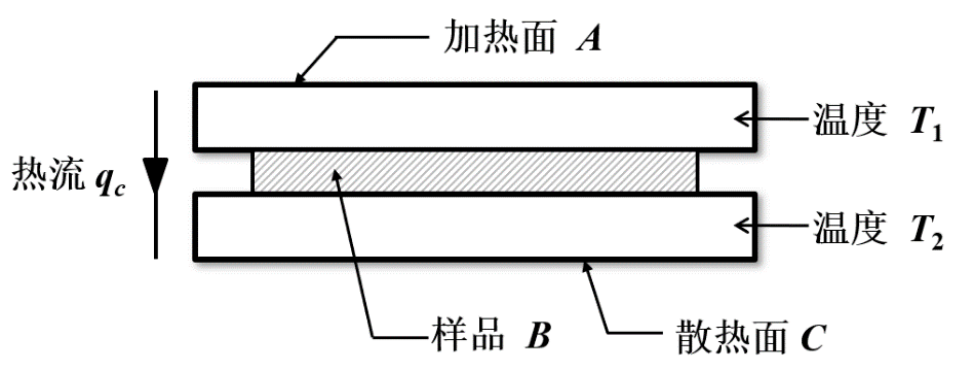
\includegraphics[width=100mm]{fg1.png}
                \caption{热流计法测量材料热导率的原理示意图 \label{fg:1}}
            \end{figure}
        \subsubsection{平面热源法测量材料热导率的原理}
            如\fgref{fg:2}所示,考虑一无穷大导热平板的一维热传导问题。假设该平板的面积为无限大、厚度为 $2d$,初始温度为 $T_0$。现从平板的两侧同时向中心面施加均匀的热流密度(单位时间通过单位截面积的热量,也被称为热通量)$q_f$(\unit{\watt\per\meter\squared}),则平板上各点的温度 $T(x,t)$ 将随加热时间 $t$而变化。
            \begin{figure}[!ht]\centering
                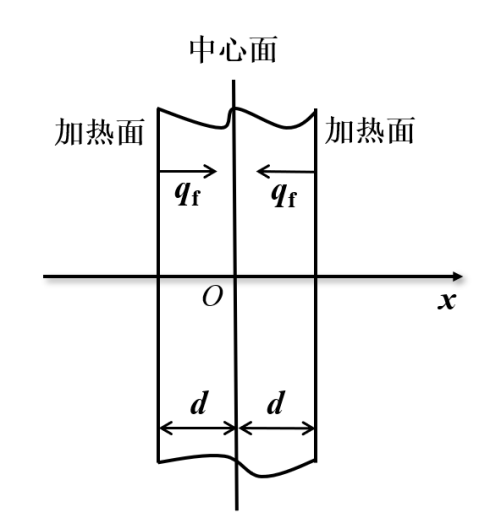
\includegraphics[width=50mm]{fg2.png}
                \caption{厚度为 $2d$ 的无穷大导热平板的一维热传导模型示意图 \label{fg:2}}
            \end{figure}\par
            以样品中心面上的一点为坐标原点 $O$,以样品厚度方向为 $x$ 轴方向,如\fgref{fg:2} 所示,则平板上各处的温度$T(x,t)$随位置 $x$和加热时间 $t$的分布可通过求解下面的偏微分方程得到:
            \begin{equation}
                \begin{cases}
                    \frac{\partial T(x,t)}{\partial t}=\alpha\frac{\partial^2T(x,t)}{\partial x^2}\\
                    \frac{\partial T(d,t)}{\partial x}=\frac{q_f}k ,\quad\frac{\partial T(0,t)}{\partial x}=0\\
                    T(x,0)=T_0
                \end{cases}
            \end{equation}
            该偏微分方程的解说明了当热流密度$q_c$恒定时,此时加热面和中心面之间的温度差$\varDelta T$保持恒定,与加热时间 $t$ 无关,我们称这种状态为准稳态。当体系到达准稳态时:\par
            \begin{equation}
                \begin{aligned}
                    k&=\frac{q_fd}{2\Delta T}\\
                    c&=\frac{q_f}{\rho d\frac{\partial T}{\partial t}}
                \end{aligned}
            \end{equation}



\section{实验仪器}%规格及参数
    DRPL-I 热导率测试仪,计算机,ZKY-BRDR 型准稳态法热导率、比热测试仪,样品(石英、白橡胶、铝合金、黑橡胶、有机玻璃)。
    \section{实验过程}%简述主要过程和实验内容
    \subsection{使用稳态法(热流计法)测量样品的热阻和材料的热导率}
    本实验使用 DRPL-I 测试仪和基于稳态测试方法的热流计法对三种样品(白橡胶、石英和铝合金)的热导率和热阻进行测试。
        \subsubsection{测量方块状白橡胶样品的热阻和白橡胶的热导率}
        \begin{enumerate}
            \item 测量样品尺寸,安装样品
            \item 设定加热温度,等到系统进入稳态后用鼠标点击“开始测量”按钮进行自动测量
            \item 测量完成后,保存数据,关机
        \end{enumerate}
        \subsubsection{测量圆柱形石英样品的热阻和石英的热导率}
        测量过程与橡胶块样品的测量过程类似,所不同的是,石英样品不像橡胶样品那样富有弹性,为了确保石英样品与上、下铜板有良好的热接触,需要在石英样品的上下底面涂抹适量的导热硅脂。
        \subsubsection{测量圆柱形铝合金样品的热阻和铝合金的热导率}
        使用游标卡尺测量铝合金样品的直径时,要注意铝合金棒的直径不包含绝热层。使用游标卡尺测量上、下两个测温孔的距离作为铝合金样品的厚度。同样地,每个量都需要测量 5 次,并将结果记录在实验记录纸上。在铝合金样品的上、下底面涂抹少量导热硅脂,然后,将样品置于铜下面板的正中央。旋转手轮,降下铜上面板使之与样品接触。用手旋转样品使导热硅脂尽可能均匀分布于两个接触面。将原来插入到上、下铜面板测温孔的热电偶测温端拔出,蘸一些导热硅脂,分别插入到样品侧面上、下两个测温孔中,而且要将热电偶的测温端插到底(插到样品中心)。旋转手轮,直到四个支撑杆露出 \SI{10}{\mm} 左右,以确保样品被上、下铜板夹紧。以下测量过程与橡胶块样品的测量过程相同。

    \subsection{使用准稳态法(平面热源法)测量有机玻璃和黑橡胶的热导率和比热}
        要使用 ZKY-BRDR 型测试仪测量材料的热导率和比热,需准备 4 块尺寸完全相同的同质样品。四块样品 1、2、3 和 4 一字排开,样品 2 和 3 之间的中央位置放置中心面热电偶测温端;样品 1 和 2 之间为面加热器1,样品 3 和 4 之间为面加热器 2,并在样品 3 和面加热器 2 之间的中央位置放置加热面热电偶测温端。测试时,四块样品和两个面加热器被紧密挤压在一起,确保样品和样品之间以及样品和加热器之间不存在空气隙,且样品和加热器周围被绝热材料所包围。由于面加热器可对整个样品面积进行均匀加热,且样品的横向尺寸大于样品厚度的 6 倍以上,可以认为热传导只沿样品厚度方向进行,所以之前在假设样品为无穷大的前提下推导出来的一维非稳态热传导公式对本实验仍然近似成立。由于面加热器可以向左、右两边加热,所以在每个面加热器的两边配置了两个相同的样品(它们具有相同的热阻),这样可使样品 2 或 3 获得的热流密度约等于面加热器一半的电功率。一旦确定了样品 2 和 3 从面加热器获得的热流密度 $q_f$ ,只需测出体系进入准稳态后加热面和中心面之间的温度差(或样品 3 两侧的温度差)$\delta T$,就可以计算材料的热导率。由于我们在样品 3 的两侧分别放置了中心面热电偶的测温端和加热面热电偶的测温端,且两个热电偶的冷端被放置在同一个保温杯中,在整个实验过程中两个热电偶的冷端温度保持恒定,所以测试过程中任意时刻样品 3 两侧的温差热电势 $V_t$(即两个热电偶的测温端温差热电势)可以由仪器测出。自然,我们便可以计算出材料的比热。
        \subsubsection{测量有机玻璃的热导率和比热}
        \begin{enumerate}
            \item 安装样品
            \item 设定加热电压
            \item 测量加热面和中心面间的温差电动势 $V_t$ 和中心面每分钟温升热电势
        \end{enumerate}
        \subsubsection{测量黑橡胶的热导率和比热}
        安装和测量黑橡胶样品的热导率和比热的操作步骤与安装和测量有机玻璃的热导率和比热的实验步骤类似,以下不再赘述。
\end{document}